\documentclass{beamer}

\usepackage{epsfig}
\usepackage{multicol}
\usepackage{geometry}
%\usepackage[dvipsnames]{xcolor}
\usepackage{textcomp}
\usepackage{graphicx}
\usepackage{caption}
\usepackage{subcaption}
\usepackage{amsmath}
\usepackage{tcolorbox}
\usetheme{Boadilla}
\usepackage{pict2e}
\usepackage{tikz}
\usepackage{xcolor}


\title[Traitement du signal numérique]{Traitement du signal numérique - HEI4 IMS}
\author[Antony Bazir]{}

\setlength{\unitlength}{1cm}

\begin{document}

\section{Outils Mathématiques}
\subsection{Transformée de Laplace}

\begin{frame}
\frametitle{Transformée de Laplace}
\textbf{Que vous évoque la transformée de Laplace ?}\\

\vspace{1cm}

\only<2->
{
	Transformée de Laplace monolatérale : $L\{f\}(s) = \displaystyle \int^{\infty}_{0} f(t) e^{-st} \; dt$\\ 
	\vspace{0.3cm}
	Transformée de Laplace bilatérale : $L\{f\}(s) = \displaystyle \int^{\infty}_{-\infty} f(t) e^{-st} \; dt$
}

\only<3->
{
\begin{block}{}
Utile, entre autre, pour analyser des systèmes dynamiques de façon rapide.
\end{block}
}

\end{frame}

\begin{frame}
\frametitle{Propriétés de la transformée de Laplace}
\begin{itemize}
\item<2-> Linéarité: \only<3->{ $L\{af+g\}(s) = a L\{ f\}(s) + L \{ g \} (s)$}
\item<4-> Dérivation : \only<5->{$ L\{f'\}(s) = \; s L\{f \}(s)$}
\item<5-> Intégration : \only<6->{$ L\{F\}(s) = \frac{\displaystyle 1}{\displaystyle s} L\{f \}(s) $}
\item<7-> Convolution : \only<8->{$ L\{f \star g \} = L\{f \}(s) \cdot L \{ g \} (s)  $}
\end{itemize}

\end{frame}

\begin{frame} 
\frametitle{Transformée de Laplace}

\textbf{Exercice: Calculer les transformées de Laplace suivantes}\\
\vspace{1cm}
\begin{itemize}
\item $u(t)$ (échelon de heaviside)
\item $r(t) = t$ (rampe)
\item $f(t) = e^{-at}$ (exponentielle décroissante)
\item $\delta (t)$ (impulsion de dirac) 
\item $sin(\omega_0 t)$
\end{itemize}

\end{frame} 

\begin{frame} 
\frametitle{Transformée de Laplace}

\textbf{Exercice: Calculer les transformées de Laplace suivantes}\\
\vspace{1cm}
\begin{itemize}
\item $u(t)$  \only<2->{$\rightarrow \frac{\displaystyle 1}{\displaystyle p} $} 
\item $r(t) = t$  \only<3->{$\rightarrow \frac{\displaystyle 1}{ \displaystyle p^2} $} 
\item $f(t) = e^{-at}$  \only<4->{$\rightarrow \frac{\displaystyle 1}{\displaystyle p+a} $}
\item $\delta (t)$ \only<5->{$\rightarrow 1$} 
\item $sin(\omega t)$ = \only<6->{$\rightarrow \frac{\displaystyle \omega_0^2}{ \displaystyle p^2 + \omega_0^2} $}
\end{itemize}

\end{frame}

\subsection{Transformée de Fourier et lien avec la transformée de Laplace}

\subsubsection{Transformée de Fourier}


\begin{frame}
\frametitle{Transformée de Fourier}
\textbf{Question: Quelle est pour vous le lien entre transformée de Laplace et transformée de Fourier}\\
\vspace{1 cm}
\only<2->
{
\begin{center}
	$L\{f\}(s) = \displaystyle \int^{\infty}_{-\infty} f(t) e^{-st} \; dt $ \only<3->{$ \rightarrow TF\{ f \}(\nu) = \displaystyle \int^{\infty}_{-\infty} f(t) e^{-j2\pi \nu t} dt $}
\end{center} 
}

\only<4->{
\begin{block}{}
La transformée de Fourier peut s'écrire commes un cas particulier de la transformée de Laplace bilatérale.
\end{block}
}
\end{frame}

\subsubsection{Spectre}
\begin{frame}
\frametitle{Transformée de Fourier}
\[ TF\{ f \}(\nu) = \displaystyle \int^{\infty}_{-\infty} f(t) e^{-j2\pi \nu t} dt   = F(\nu) \]\\
\vspace{1cm}

La fonction $F(\nu)$ est généralement désigné comme \textbf{spectre fréquentiel} de $f(t)$ \\

\vspace{1cm}
\only<2->{
$F(\nu)$ est une fonction \textbf{complexe} 
}

\only<3->{
\begin{block}{}
Comment le représenter ? 
\end{block}
}
\end{frame}

\begin{frame}
\frametitle{Transformée de Fourier : Spectre }

Comment représenter $F(\nu)$  ? \\

\vspace{1cm} 

2 possibilités pour représenter un nombre complexe $z$: 

\begin{itemize}
\item $z = a+ ib$
\item $z = r\cdot e^{i \theta}$
\end{itemize} 

\vspace{1 cm}

\only<2->{
\begin{block}{}
Dans la grande majorité des cas c'est la représentation module/argument $z = r\cdot e^{i \theta}$ qui est utilisée.
\end{block}
}

\subsubsection{Module et phase: exemples}

\vspace{1cm}
\only<3->
{
On va prendre la fonction $g_1(t) = \cos(2 t)$ pour illustrer
}

\end{frame} 

\begin{frame}
\frametitle{Transformée  de Fourier : Spectre}
Spectre de $g_1(t) = \cos(2 t)$ \\

\only<2->{
\begin{center}
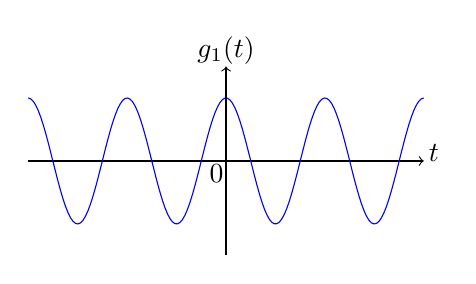
\begin{tikzpicture}
\begin{scope}[scale=0.4]
	\draw[->] (-6.28,0)-- (6.28,0);
\draw (-0.3,-0.4) node {0};
\draw[->] (0,-3)-- (0,3);
\draw (2.1*pi,0.25) node {$t$};
\draw (0,3.5) node {$g_1(t)$};

\draw[domain=-6.28:6.28,color=blue,samples=160] plot (\x,{2*cos(2*\x r)});	
\end{scope}
\end{tikzpicture}
\end{center}
}

\only<3->{
Soit $z = a +ib$, alors $|z|=$\only<2->{$r = \sqrt{a^2 + b^2}$}
et $arg(z) = \theta = \arctan(\frac{\displaystyle b}{\displaystyle a})$
}

\vspace{0.4 cm} 

\only<4->{
 $$TF\{ g_1 \}(\nu) = \int^{\infty}_{-\infty} g_1(t) e^{-2\pi j \nu t} \; dt$$ \only<5->{$$= \frac{\displaystyle \delta(\nu - 1/\pi) + \delta(\nu + 1/\pi)}{\displaystyle 2}
$$}}

\end{frame}

\begin{frame}
\frametitle{Transformée  de Fourier : Spectre}
 $$TF\{ g_1 \}(\nu) = \int^{\infty}_{-\infty} g_1(t) e^{-2\pi j \nu t} \; dt= \frac{\displaystyle \delta(\nu - 1/\pi) + \delta(\nu + 1/\pi)}{\displaystyle 2}$$\\
 
 \vspace{1cm}
 \only<2->{
 $$|TF\{ g_1 \}(\nu)| = |G_1(\nu)| = \frac{\displaystyle \delta(\nu - 1/\pi) + \delta(\nu + 1/\pi)}{\displaystyle 2} $$
 }
 
\only<3->{
\begin{center}
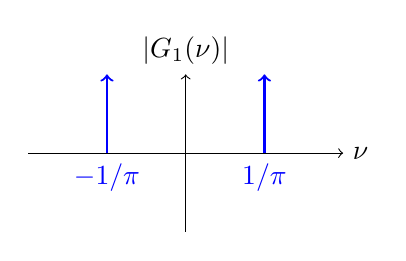
\begin{tikzpicture}
\draw[->] (-2,0)--(2,0) node[right]{$\nu$};
\draw[->] (0,-1)--(0,1) node[above]{$|G_1(\nu)|$};
\draw[->,blue,thick] (-1,0) node[below]{$-1/\pi$}--(-1,1) ;
\draw[->,blue,thick] (1,0) node[below]{$1/\pi$}--(1,1) ;
\end{tikzpicture}
\end{center}
}
\end{frame}

\begin{frame}
\frametitle{Transformée de Fourier : Spectre}
$$G_1(\nu) = \frac{\displaystyle \delta(\nu - 1/\pi) + \delta(\nu + 1/\pi)}{\displaystyle 2} $$\\

\vspace{0.6cm}
\only<2->{
$$arg(G_1(\nu)) = $$ \only<3->{ $$\arctan(\frac{0}{\frac{\displaystyle \delta(\nu - 1/\pi) + \delta(\nu + 1/\pi)}{\displaystyle 2}}) = 0$$}\\
}
\vspace{0.6cm}
\only<3->{
\begin{center}
\begin{tikzpicture}
\draw[->] (-2,0)--(2,0) node[right]{$\nu$};
\draw[->] (0,-1)--(0,1) node[above]{$arg(G_1(\nu))$};
\draw[->,blue,thick] (-1,0) node[below]{$-1/\pi$}--(-1,0) ;
\draw[->,blue,thick] (1,0) node[below]{$1/\pi$}--(1,0) ;
\end{tikzpicture}
\end{center}
}

\end{frame}

\begin{frame}
\frametitle{Transformée  de Fourier : Spectre}
En résumé, \\
\vspace{0.3cm}
\[g_1(t) = \cos(2 t) \rightarrow  G_1(\nu) = \frac{\displaystyle \delta(\nu - 1/\pi) + \delta(\nu + 1/\pi)}{\displaystyle 2} \]

\begin{columns}
\column{60mm}
\only<2->{
\[|G_1(\nu)| = \frac{\displaystyle \delta(\nu - 1/\pi) + \delta(\nu + 1/\pi)}{\displaystyle 2}\]\\
}
\vspace{0.1cm}
\only<3->
{
\begin{center}
\begin{tikzpicture}
\draw[->] (-2,0)--(2,0) node[right]{$\nu$};
\draw[->] (0,-1)--(0,1) node[above]{$|G_1(\nu)|$};
\draw[->,blue,thick] (-1,0) node[below]{\scriptsize $-1/\pi$}--(-1,1) ;
\draw[->,blue,thick] (1,0) node[below]{\scriptsize $1/\pi$}--(1,1) ;
\end{tikzpicture}
\end{center}
}

\column{60mm}
\only<2->{
$$arg(G_1(\nu))  = 0 $$ \\
}
\vspace{0.65cm}
\only<3->
{
\begin{center}
\begin{tikzpicture}
\draw[->] (-2,0)--(2,0) node[right]{$\nu$};
\draw[->] (0,-1)--(0,1) node[above]{$arg(G_1(\nu))$};
\draw[->,blue,thick] (-1,0) node[below]{\scriptsize $-1/\pi$}--(-1,0) ;
\draw[->,blue,thick] (1,0) node[below]{ \scriptsize $1/\pi$}--(1,0) ;
\end{tikzpicture}
\end{center}
}
\end{columns}
\end{frame}

\begin{frame}
\frametitle{Transformée  de Fourier : Spectre}
Spectre de $g_2(t) = 0.55\cos(2 t) + 0.45 \cos(4 t + \frac{\pi}{3})$ \\
\only<2->{
\begin{center}
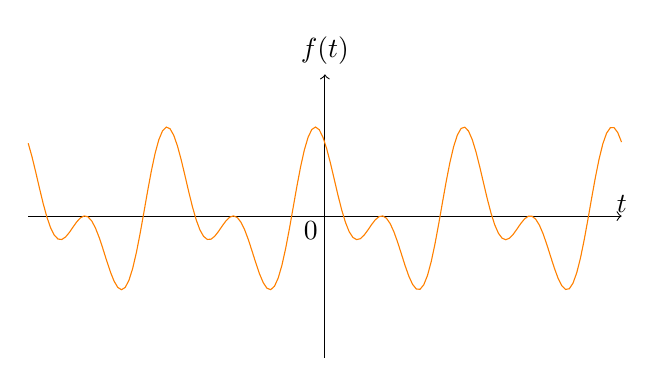
\begin{tikzpicture}
\begin{scope}[scale=0.6]
	\draw[->] (-6.28,0)-- (6.28,0);
\draw (-0.3,-0.3) node {0};
\draw[->] (0,-3)-- (0,3);
\draw (2*pi,0.25) node {$t$};
\draw (0,3.5) node {$f(t)$};
%\draw (4.5,-0.3) node {1};

		\draw[domain=-6.28:6.28,color=orange,samples=160] plot (\x,{2*(0.55*cos(2*\x r)+ 0.45*cos(2*2*(\x+3.14/12) r))});
	\end{scope}
	\end{tikzpicture}
\end{center}
}
\end{frame}

\begin{frame}
\frametitle{Transformée  de Fourier : Spectre}

\[ TF\{ g_2 \}(f) = G_2(\nu)\]\\
\[ =   \frac{0.55}{2}(\delta(\nu+1/\pi) + \delta(\nu-1/\pi)) + \frac{0.45}{2}(\delta(\nu+2/\pi) + \delta(\nu-2/\pi)) \cdot e^{2 j \pi \frac{\pi}{3} \nu }\]\\

\vspace{0.5 cm}

\[|G_2(\nu)| = \bigl[(\frac{0.55}{2}(\delta(\nu+1/\pi) + \delta(\nu-1/\pi))+ \] \\
\[ \frac{0.45}{2}(\delta(\nu+2/\pi) + \delta(\nu-2/\pi)) \cdot  \cos(2\frac{\pi^2}{3} \nu))^2 \]\\
\[+(\frac{0.45}{2}(\delta(\nu+2/\pi) + \delta(\nu-2/\pi)) \cdot  \sin(2\frac{\pi^2}{3} \nu))^2 \bigr] ^{1/2} \]

\end{frame}

\begin{frame} 
\frametitle{Transformée  de Fourier : Spectre}

\[|G_2(\nu)| = \bigl[(\frac{0.55}{2}(\delta(\nu+1/\pi) + \delta(\nu-1/\pi))+ \] \\
\[ \frac{0.45}{2}(\delta(\nu+2/\pi) + \delta(\nu-2/\pi)) \cdot  \cos(2\frac{\pi^2}{3} \nu))^2 \]\\
\[+(\frac{0.45}{2}(\delta(\nu+2/\pi) + \delta(\nu-2/\pi)) \cdot  \sin(2\frac{\pi^2}{3} \nu))^2 \bigr] ^{1/2} \]\\

\vspace{0.5cm}
\only<2->{
\begin{center}
\begin{tikzpicture}
\draw[->] (-2.5,0)--(2.5,0) node[right]{$\nu$};
\draw[->] (0,-1)--(0,1) node[above]{$|G_2(\nu)|$};
\draw[->,orange,thick] (-1,0) node[below]{\scriptsize $-1/\pi$}--(-1,0.55) ;
\draw[->,orange,thick] (1,0) node[below]{\scriptsize $1/\pi$}--(1,0.55) ;
\draw[->,orange,thick] (-2,0) node[below]{\scriptsize $-2/\pi$}--(-2,0.225) ;
\draw[->,orange,thick] (2,0) node[below]{\scriptsize $2/\pi$}--(2,0.225) ;
\end{tikzpicture}
\end{center}
}
\end{frame}

\begin{frame}
\frametitle{Transformée  de Fourier : Spectre}
\[ arg(G_2(\nu)) = \]\\
\[ \arctan\bigl( \frac{\frac{0.45}{2}(\delta_2) \cdot  \sin(2\frac{\pi^2}{3} \nu)}{\frac{0.55}{2}(\delta_1)+
 \frac{0.45}{2}(\delta_2) \cdot  \cos(2\frac{\pi^2}{3} \nu)}\bigr) \]\\
 \vspace{0.3cm} 
 \only<2->{
 \[arg(G_2(\nu)) = 2\frac{\pi^2}{3} \nu*\delta_2 \]\\
 }

 \vspace{0.3cm}
 \only<3->
{
\begin{center}
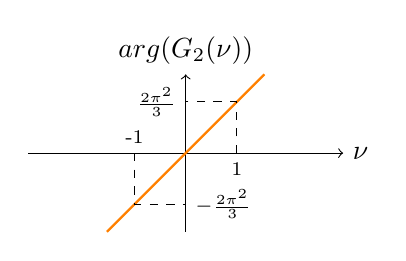
\begin{tikzpicture}
\draw[->] (-2,0)--(2,0) node[right]{$\nu$};
\draw[->] (0,-1)--(0,1) node[above]{$arg(G_2(\nu))$};
\draw[orange,thick] (-1,-1) --(1,1) ;
\draw[dashed] (-0.65,0)node[above]{\scriptsize -1} --(-0.65,-0.65)--(0,-0.65)node[right]{\scriptsize $-\frac{2\pi^2}{3}$} ;
\draw[dashed] (0.65,0)node[below]{\scriptsize 1} --(0.65,0.65)--(0,0.65)node[left]{\scriptsize $\frac{2\pi^2}{3}$} ;
\end{tikzpicture}
\end{center}
}
\end{frame}

\begin{frame}
\frametitle{Transformée  de Fourier : Spectre}
\[ TF\{ g_2 \}(f) = G_2(\nu)\]\\
\[ =   \frac{0.55}{2}(\delta(\nu+1/\pi) + \delta(\nu-1/\pi)) + \frac{0.45}{2}(\delta(\nu+2/\pi) + \delta(\nu-2/\pi)) \cdot e^{2 j \pi \frac{\pi}{3} \nu }\]\\

\vspace{0.3cm}
\begin{columns}
\column{60mm}
\only<2->{
\begin{center}
\begin{tikzpicture}
\draw[->] (-2.5,0)--(2.5,0) node[right]{$\nu$};
\draw[->] (0,-1)--(0,1) node[above]{$|G_2(\nu)|$};
\draw[->,orange,thick] (-1,0) node[below]{\scriptsize $-1/\pi$}--(-1,0.55) ;
\draw[->,orange,thick] (1,0) node[below]{\scriptsize $1/\pi$}--(1,0.55) ;
\draw[->,orange,thick] (-2,0) node[below]{\scriptsize $-2/\pi$}--(-2,0.225) ;
\draw[->,orange,thick] (2,0) node[below]{\scriptsize $2/\pi$}--(2,0.225) ;
\end{tikzpicture}
\end{center}

}
\column{60mm}
\only<2->{
\begin{center}
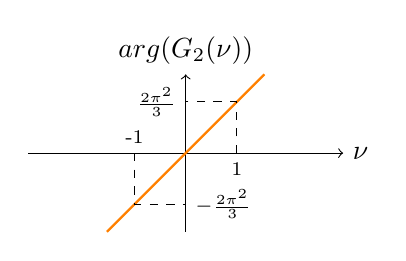
\begin{tikzpicture}
\draw[->] (-2,0)--(2,0) node[right]{$\nu$};
\draw[->] (0,-1)--(0,1) node[above]{$arg(G_2(\nu))$};
\draw[orange,thick] (-1,-1) --(1,1) ;
\draw[dashed] (-0.65,0)node[above]{\scriptsize -1} --(-0.65,-0.65)--(0,-0.65)node[right]{\scriptsize $-\frac{2\pi^2}{3}$} ;
\draw[dashed] (0.65,0)node[below]{\scriptsize 1} --(0.65,0.65)--(0,0.65)node[left]{\scriptsize $\frac{2\pi^2}{3}$} ;
\end{tikzpicture}
\end{center}

}

\end{columns}

\end{frame}

\begin{frame}
\frametitle{Transformée  de Fourier : Spectre}
La phase a son importance... \\
\vspace{0.3cm}
Si on prend  $g_3(t) = 0.55\cos(2 t) + 0.45 \cos(4 t)$...\\
\vspace{0.3cm}
\begin{columns}
\column{60mm}
\only<2->{



\begin{center}
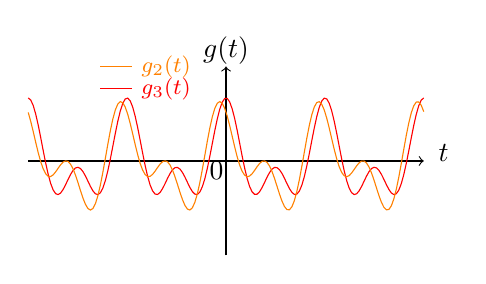
\begin{tikzpicture}
	\begin{scope}[scale=0.4]
	\draw[->] (-6.28,0)-- (6.28,0);
\draw (-0.3,-0.3) node {0};
\draw[->] (0,-3)-- (0,3);
\draw (2.2*pi,0.25) node {$t$};
\draw (0,3.5) node {$g(t)$};

	\draw[domain=-6.28:6.28,color=red,samples=160] plot (\x,{2*(0.55*cos(2*\x r)+ 0.45*cos(2*2*\x r))});
	
		\draw[domain=-6.28:6.28,color=orange,samples=160] plot (\x,{2*(0.55*cos(2*\x r)+ 0.45*cos(2*2*(\x+3.14/12) r))});
		
		\draw[orange] (-4,3)--(-3,3)node[right] {\footnotesize $g_2(t)$};
		\draw[red] (-4,2.3)--(-3,2.3)node[right] {\footnotesize $g_3(t)$};
	\end{scope}
	\end{tikzpicture}
\end{center}


\only<4->
{
L'ajout d'un déphasage à une des composantes change la forme du signal et la phase (qui devient nulle) mais PAS le module
}

\column{60mm}
\only<3->{
\begin{center}
\begin{tikzpicture}
\draw[->] (-2.5,0)--(2.5,0) node[right]{$\nu$};
\draw[->] (0,-1)--(0,1) node[above]{$|G_3(\nu)|$};
\draw[->,red,thick] (-1,0) node[below]{\scriptsize $-1/\pi$}--(-1,0.55) ;
\draw[->,red,thick] (1,0) node[below]{\scriptsize $1/\pi$}--(1,0.55) ;
\draw[->,red,thick] (-2,0) node[below]{\scriptsize $-2/\pi$}--(-2,0.225) ;
\draw[->,red,thick] (2,0) node[below]{\scriptsize $2/\pi$}--(2,0.225) ;
\end{tikzpicture}
\end{center}
\vspace{0cm}
\begin{center}
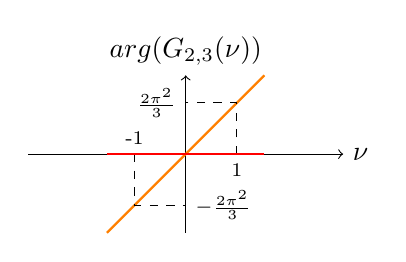
\begin{tikzpicture}
\draw[->] (-2,0)--(2,0) node[right]{$\nu$};
\draw[->] (0,-1)--(0,1) node[above]{$arg(G_{2,3}(\nu))$};
\draw[orange,thick] (-1,-1) --(1,1) ;
\draw[dashed] (-0.65,0)node[above]{\scriptsize -1} --(-0.65,-0.65)--(0,-0.65)node[right]{\scriptsize $-\frac{2\pi^2}{3}$} ;
\draw[dashed] (0.65,0)node[below]{\scriptsize 1} --(0.65,0.65)--(0,0.65)node[left]{\scriptsize $\frac{2\pi^2}{3}$} ;
\draw[red,thick] (-1,0) --(1,0) ;
\end{tikzpicture}
\end{center}
}
} 
\end{columns}
\vspace{0.3cm}

\end{frame}

\subsection{Concepts utile dans le domaine de Fourier}

\begin{frame}
\frametitle{Choses à savoir sur la Transformée de Fourier}
Il y a des petites "lois" qu'il peut être utile d'avoir à l'esprit lorsqu'on manipule des fonctions et leurs spectres...\\

\vspace{0.1cm}
\only<2->
{
1a.\textbf{ Extension temporelle faible = Extension fréquentielle forte}
}

\only<3->{
\begin{center}
\begin{tikzpicture}
\draw[->] (-2,0)--(2,0) node[right]{$t$};
\draw[->] (0,-1)--(0,1) node[above]{$f(t)$};
\draw[thick,blue] (-2,0)--(0,0)--(0,1)--(0,0)--(2,0);

\begin{scope}[xshift=6cm]
\draw[->] (-2,0)--(2,0) node[right]{$\nu$};
\draw[->] (0,-1)--(0,1) node[above]{$F(\nu)$};
\draw[thick,blue] (-2,0.5)--(2,0.5);
\end{scope}
\end{tikzpicture}
\end{center}
}

\only<4->
{
1b.\textbf{ Extension temporelle forte = Extension fréquentielle faible}
}

\only<4->{
\begin{center}
\begin{tikzpicture}
\draw[->] (-2,0)--(2,0) node[right]{$t$};
\draw[->] (0,-1)--(0,1) node[above]{$f(t)$};
\draw[thick,blue] (-2,0.5)--(2,0.5);

\begin{scope}[xshift=6cm]
\draw[->] (-2,0)--(2,0) node[right]{$\nu$};
\draw[->] (0,-1)--(0,1) node[above]{$F(\nu)$};
\draw[thick,blue] (-2,0)--(0,0)--(0,1)--(0,0)--(2,0);
\end{scope}
\end{tikzpicture}
\end{center}
}

\end{frame} 

\begin{frame}
\frametitle{Choses à savoir sur la Transformée de Fourier}
2. Périodicité temporelle et spectre 


\only<2->{
\begin{tikzpicture}
\draw[->] (2.5,0) node[below] {0} -- (2.5,1.5)node[above] {$e(t)$};
\draw[->] (0,0)-- (5,0) node[right] {$t$};

\draw[thick,blue] (2,0)--(2.25,0)--(2.25,1)--(2.75,1)--(2.75,0)--(3,0);

\begin{scope}[xshift=1cm]
\draw[thick,blue] (2,0)--(2.25,0)--(2.25,1)--(2.75,1)--(2.75,0)--(3,0);
\draw[dashed,black] (2.5,0) node[below]{$T$}--(2.5,1);
\end{scope}

\begin{scope}[xshift=2cm]
\draw[thick,blue] (2,0)--(2.25,0)--(2.25,1)--(2.75,1)--(2.75,0)--(3,0);
\end{scope}


\begin{scope}[xshift=-1cm]
\draw[thick,blue] (2,0)--(2.25,0)--(2.25,1)--(2.75,1)--(2.75,0)--(3,0);
\end{scope}

\begin{scope}[xshift=-2cm]
\draw[thick,blue] (2,0)--(2.25,0)--(2.25,1)--(2.75,1)--(2.75,0)--(3,0);
\end{scope}



\begin{scope}[xshift=7cm]
\draw[->] (2.5,0) node[below] {0} -- (2.5,1.5)node[above] {$E(\nu)$};
\draw[->] (0,0)-- (5,0) node[right] {$\nu$};
\draw[ domain=0.1:4.9,color=blue,samples=24] plot[ycomb] (\x,{80*abs(sin(5*3.14*\x r -5*3.14*2.5r )/(5*3.14*\x r-5*3.14*2.5 r))});
\draw[<->] (3.25,-0.3)--(3.45,-0.3) node[below left] {$\frac{1}{T}$};
\end{scope}
\end{tikzpicture}
}

\only<3->{
\begin{tikzpicture}
\draw[->] (2.5,0) node[below] {0} -- (2.5,1.5)node[above] {$e(t)$};
\draw[->] (0,0)-- (5,0) node[below right] {$t$};

\draw[thick,blue] (1,0)--(2.25,0)--(2.25,1)--(2.75,1)--(2.75,0)--(4,0);


\begin{scope}[xshift=2cm]
\draw[thick,blue] (1,0)--(2.25,0)--(2.25,1)--(2.75,1)--(2.75,0)--(3,0);
\end{scope}


\begin{scope}[xshift=-2cm]
\draw[thick,blue] (2,0)--(2.25,0)--(2.25,1)--(2.75,1)--(2.75,0)--(4,0);
\end{scope}



\begin{scope}[xshift=7cm]
\draw[->] (2.5,0) node[below] {0} -- (2.5,1.5)node[above] {$E(\nu)$};
\draw[->] (0,0)-- (5,0) node[right] {$\nu$};
\draw[ domain=0.1:4.9,color=blue,samples=96] plot[ycomb] (\x,{80*abs(sin(5*3.14*\x r -5*3.14*2.5r )/(5*3.14*\x r-5*3.14*2.5 r))});
%\draw[<->] (3.25,-0.3)--(3.45,-0.3) node[below left] {$\frac{1}{T}$};
\end{scope}
\end{tikzpicture}
}

\only<4->{
Pertinent lorsqu'il est question d'échantillonnage...
}
\end{frame}


\end{document}